\documentclass[a4paper,12pt]{article}
\usepackage{czech}
\usepackage[utf8]{inputenc}
\usepackage{a4wide}
\usepackage[dvipdfm]{graphicx}
\usepackage{graphics}
\usepackage{indentfirst}
\usepackage{fancyhdr}
\usepackage{setspace}
\usepackage{amsmath}
\usepackage{amssymb}
\usepackage{epsfig}

%%\usepackage{nopageno}
%%\usepackage{txfonts}
\usepackage[usenames]{color}
\begin{document}

\section{Úkol}
\begin{enumerate}
\item Změřte charakteristiku Geigrova-Müllerova detektoru pro záření gamma a u jednotlivých měření stanovte chybu a vyznačte ji do grafu. Určete délku a sklon plata v charakteristice detektoru a diskutujte přesnosti v určení těchto veličin.
\item Změřte mrtvou dobu detektoru metodou dvou zářičů a stanovne chybu měření
\item Studujte počty naměřených impulsů v různých časových intervalech. Srovnejte jejich rozdělení s Poissonovým, respektive Gaussovým rodělením.
\item Změřte intenzitu záření pro dvě různé vzdálenosti zářiče od detektoru a určete v obou případech dobu, po kterou je nutno měřit (intenzitu i pozadí), aby byla dosažena statistická přesnost 1 \%.
\end{enumerate}

\section{Teorie}
\subsection{Geiger-Müllerův počítač}
Geiger-Müllerův počítač je plynový detektor k určování intenzity radiaktivního záření. V principu se jedná k kondenzátor naplněný vhodným plynem, na který je přivedeno vysoké napětí a a proudový impulz odpovídá průletu radioaktivní částice.

\subsection{Mrtvá doba detektoru}
Mrtvá doba detektoru je podrobně probrána v \cite{text}. Pro účely úkolu 2 stačí znát vzorec
\begin{eqnarray}
\tau=\tau_1\left[1+\frac{\tau_1}{2}(n_{12}-n_p)\right]
\label{md}
\end{eqnarray}
,kde
\begin{eqnarray}
\tau_1=\frac{n_1+n_2-n_{12}-n_p}{2(n_1-n_p)(n_2-n_p)}
\end{eqnarray}

\section{Měření}
\subsection{Geiger-Müllerova charakteristika}
Nejpreve jsem proměřil Geiger-Müllerovu charakteristiku detektoru. Doba měření byla 40 s.
Výsledky jsou v tabulce \ref{T1}. Výsledná charakteristika je na obrázku \ref{g1}.

Plato začíná okolo napětí 350 V a na jeho konec jsem do limitu napětí, kterým bylo 460 
V nenarazil. Proložená přímka nám dáva jeho sklon
\begin{eqnarray}
k=(2.66\pm 0.48) \mbox{V}^{-1}
\end{eqnarray}
Gnuplot určil chybu skolu fitu 18 \%.

\begin{table}
$$
\begin{array}{|c|c|}
\hline
U/\mbox{V}& N \\ \hline
125&0\pm0\\ \hline
270&0\pm0\\ \hline
286&0\pm0\\ \hline
294&4704\pm69\\ \hline
302&5159\pm72\\ \hline
310&5099\pm71\\ \hline
318&5176\pm72\\ \hline
326&8349\pm91\\ \hline
330&5300\pm73\\ \hline
334&5222\pm72\\ \hline
338&4994\pm71\\ \hline
342&4676\pm68\\ \hline
346&4890\pm70\\ \hline
354&4915\pm70\\ \hline
362&4847\pm70\\ \hline
370&4868\pm70\\ \hline
378&4953\pm70\\ \hline
386&4996\pm71\\ \hline
394&5009\pm71\\ \hline
400&4993\pm71\\ \hline
402&4980\pm71\\ \hline
408&5006\pm71\\ \hline
416&5001\pm71\\ \hline
424&5197\pm72\\ \hline
432&5079\pm71\\ \hline
440&5066\pm71\\ \hline
448&5097\pm71\\ \hline
456&5100\pm71\\ \hline
\end{array}
$$
\caption{Hodnoty Gagier-Müllerovy charakteristiky}
\label{T1}
\end{table}

\begin{figure}
\begin{center}
% GNUPLOT: LaTeX picture with Postscript
\begingroup
  \makeatletter
  \providecommand\color[2][]{%
    \GenericError{(gnuplot) \space\space\space\@spaces}{%
      Package color not loaded in conjunction with
      terminal option `colourtext'%
    }{See the gnuplot documentation for explanation.%
    }{Either use 'blacktext' in gnuplot or load the package
      color.sty in LaTeX.}%
    \renewcommand\color[2][]{}%
  }%
  \providecommand\includegraphics[2][]{%
    \GenericError{(gnuplot) \space\space\space\@spaces}{%
      Package graphicx or graphics not loaded%
    }{See the gnuplot documentation for explanation.%
    }{The gnuplot epslatex terminal needs graphicx.sty or graphics.sty.}%
    \renewcommand\includegraphics[2][]{}%
  }%
  \providecommand\rotatebox[2]{#2}%
  \@ifundefined{ifGPcolor}{%
    \newif\ifGPcolor
    \GPcolorfalse
  }{}%
  \@ifundefined{ifGPblacktext}{%
    \newif\ifGPblacktext
    \GPblacktexttrue
  }{}%
  % define a \g@addto@macro without @ in the name:
  \let\gplgaddtomacro\g@addto@macro
  % define empty templates for all commands taking text:
  \gdef\gplbacktext{}%
  \gdef\gplfronttext{}%
  \makeatother
  \ifGPblacktext
    % no textcolor at all
    \def\colorrgb#1{}%
    \def\colorgray#1{}%
  \else
    % gray or color?
    \ifGPcolor
      \def\colorrgb#1{\color[rgb]{#1}}%
      \def\colorgray#1{\color[gray]{#1}}%
      \expandafter\def\csname LTw\endcsname{\color{white}}%
      \expandafter\def\csname LTb\endcsname{\color{black}}%
      \expandafter\def\csname LTa\endcsname{\color{black}}%
      \expandafter\def\csname LT0\endcsname{\color[rgb]{1,0,0}}%
      \expandafter\def\csname LT1\endcsname{\color[rgb]{0,1,0}}%
      \expandafter\def\csname LT2\endcsname{\color[rgb]{0,0,1}}%
      \expandafter\def\csname LT3\endcsname{\color[rgb]{1,0,1}}%
      \expandafter\def\csname LT4\endcsname{\color[rgb]{0,1,1}}%
      \expandafter\def\csname LT5\endcsname{\color[rgb]{1,1,0}}%
      \expandafter\def\csname LT6\endcsname{\color[rgb]{0,0,0}}%
      \expandafter\def\csname LT7\endcsname{\color[rgb]{1,0.3,0}}%
      \expandafter\def\csname LT8\endcsname{\color[rgb]{0.5,0.5,0.5}}%
    \else
      % gray
      \def\colorrgb#1{\color{black}}%
      \def\colorgray#1{\color[gray]{#1}}%
      \expandafter\def\csname LTw\endcsname{\color{white}}%
      \expandafter\def\csname LTb\endcsname{\color{black}}%
      \expandafter\def\csname LTa\endcsname{\color{black}}%
      \expandafter\def\csname LT0\endcsname{\color{black}}%
      \expandafter\def\csname LT1\endcsname{\color{black}}%
      \expandafter\def\csname LT2\endcsname{\color{black}}%
      \expandafter\def\csname LT3\endcsname{\color{black}}%
      \expandafter\def\csname LT4\endcsname{\color{black}}%
      \expandafter\def\csname LT5\endcsname{\color{black}}%
      \expandafter\def\csname LT6\endcsname{\color{black}}%
      \expandafter\def\csname LT7\endcsname{\color{black}}%
      \expandafter\def\csname LT8\endcsname{\color{black}}%
    \fi
  \fi
  \setlength{\unitlength}{0.0500bp}%
  \begin{picture}(7200.00,5040.00)%
    \gplgaddtomacro\gplbacktext{%
      \csname LTb\endcsname%
      \put(1210,704){\makebox(0,0)[r]{\strut{} 700}}%
      \put(1210,1074){\makebox(0,0)[r]{\strut{} 800}}%
      \put(1210,1444){\makebox(0,0)[r]{\strut{} 900}}%
      \put(1210,1814){\makebox(0,0)[r]{\strut{} 1000}}%
      \put(1210,2184){\makebox(0,0)[r]{\strut{} 1100}}%
      \put(1210,2554){\makebox(0,0)[r]{\strut{} 1200}}%
      \put(1210,2925){\makebox(0,0)[r]{\strut{} 1300}}%
      \put(1210,3295){\makebox(0,0)[r]{\strut{} 1400}}%
      \put(1210,3665){\makebox(0,0)[r]{\strut{} 1500}}%
      \put(1210,4035){\makebox(0,0)[r]{\strut{} 1600}}%
      \put(1210,4405){\makebox(0,0)[r]{\strut{} 1700}}%
      \put(1210,4775){\makebox(0,0)[r]{\strut{} 1800}}%
      \put(1342,484){\makebox(0,0){\strut{} 0}}%
      \put(2263,484){\makebox(0,0){\strut{} 0.5}}%
      \put(3184,484){\makebox(0,0){\strut{} 1}}%
      \put(4105,484){\makebox(0,0){\strut{} 1.5}}%
      \put(5027,484){\makebox(0,0){\strut{} 2}}%
      \put(5948,484){\makebox(0,0){\strut{} 2.5}}%
      \put(6869,484){\makebox(0,0){\strut{} 3}}%
      \put(308,2739){\rotatebox{-270}{\makebox(0,0){\strut{}$h$/keV$\cdot$m$^{-1}$}}}%
      \put(4105,154){\makebox(0,0){\strut{}$x$/cm}}%
    }%
    \gplgaddtomacro\gplfronttext{%
    }%
    \gplbacktext
    \put(0,0){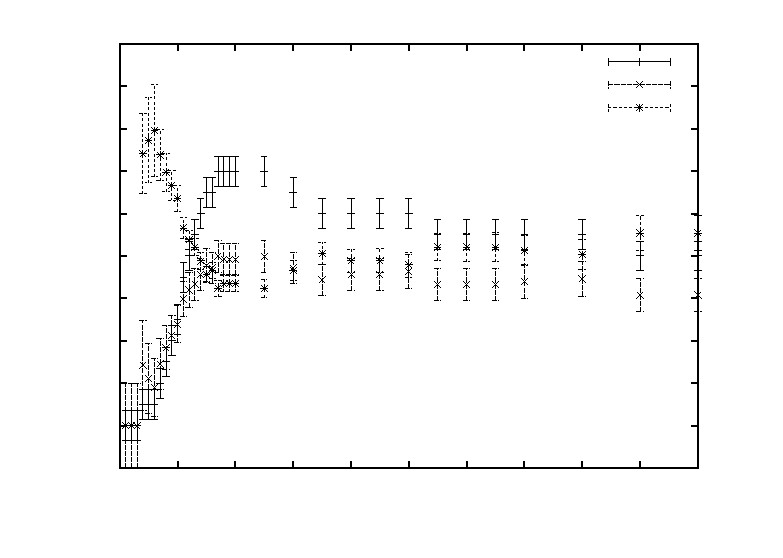
\includegraphics{g1}}%
    \gplfronttext
  \end{picture}%
\endgroup

\end{center}
\caption{Geiger-Müllerova charakteristika}
\label{g1}
\end{figure}

\subsection{Mrtvá doba}
Metodou dvou zářičů popsanou v \cite{text} jsem určoval mrtvou dobu detektoru. 
Naměřené hodnoty za 400 s byli
\begin{eqnarray}
N_{p1}=758\\
N_1=50458\\
N_{12}=67329\\
N_2=20167\\
N_{p2}=781
\end{eqnarray}
Ze vzorce \ref{md} jsem dopočítal mrtvou dobu detektoru
\begin{eqnarray}
\tau=(5.47\pm 0.13)\cdot 10^{-4} \mbox{s}
\end{eqnarray}
Relativní chyba měření je 2 \%.

\subsection{Rozdělení}
Proměřil jsem počty neměřených impulsů pro intervaly 30, 50, 100, 800 a 1000 ms. 
Tyto hodnoty jsem proložil Gaussovým rozdělením a výsledky jsou na obrázcích 
\ref{gm30} až \ref{gm1000}. Z frafů je dobře vidět, jak kratši intervaly lépe sedí 
na křivce.

\begin{figure}
\begin{center}
\input{gm30.tex}
\end{center}
\caption{Rozdělení počtu detekovaných impulsů pro interval 30 ms.}
\label{gm30}
\end{figure}

\begin{figure}
\begin{center}
\input{gm50.tex}
\end{center}
\caption{Rozdělení počtu detekovaných impulsů pro interval 50 ms.}
\label{gm50}
\end{figure}

\begin{figure}
\begin{center}
\input{gm100.tex}
\end{center}
\caption{Rozdělení počtu detekovaných impulsů pro interval 100 ms.}
\label{gm100}
\end{figure}


\begin{figure}
\begin{center}
\input{gm800.tex}
\end{center}
\caption{Rozdělení počtu detekovaných impulsů pro interval 800 ms.}
\label{gm800}
\end{figure}


\begin{figure}
\begin{center}
\input{gm1000.tex}
\end{center}
\caption{Rozdělení počtu detekovaných impulsů pro interval 1000 ms.}
\label{gm1000}
\end{figure}

\subsection{Závislost intenzity na vzdálenosti}
Za 400 s jsem přímo pod detektorem naměřil
\begin{eqnarray}
N=20167
\end{eqnarray}
Ve vzdálenosti přibližně 7 cm jsem poté za stejnou dobu naměřil
\begin{eqnarray}
N=9567
\end{eqnarray}
Aby chyba měření byla 1 \% musím detekovat 10000 interakcí. Tohoto čísla bych dosáhl po
200 reps. 419 sekundách.

\section{Diskuze}
Při proměřování Geiger-Müllerovy charakteristiky jsem objevil pík na napětí 326 V. 
Bohužel však neznám jeho fyzikální vysvětlení. Zbytek charakteristiky už odpovídal teorii. 

Při měření mrtvé doby detektoru byla velmi dobře zvolena doba měření, takže celková 
chyba vyšla velmi dobře. Konkrétně 2 \%.

Při studiu rozložení počtu detekovaných impulzů za různých časových intervalů je dobře vidět přechod od Poissonova ke Gaussovu rozložení.

\section{Závěr}
Změřil jsem Geiger-Müllerovu charakteristiku detektoru. Výsledky jsou v tabulce \ref{T1} a na obrázku \ref{g1}. \\
Změřil jsem mrtvou dobu detektoru
\begin{eqnarray}
\tau=(5.47\pm 0.13)\cdot 10^{-4} \mbox{s}
\end{eqnarray}
Studoval jsem počty naměřených impulsů pro různé časové intervaly. Výsledky jsou na obrázcích \ref{gm30} až \ref{gm1000}.
Změřil jsem intenzitu záření pro dvě různé vzdálenosti vzorku. Pro získání přesnoti 1 \% pro vzorek u respektive 7 cm od detektoru je třeba měřil 200 resp. 418 s.

\begin{thebibliography}{5}
	\bibitem{text} \textbf{Studijní text na praktikum IV} \\http://physics.mff.cuni.cz/vyuka/zfp/txt\_414.pdf (3. 11. 2012)
    \bibitem{chyba} \emph{J. Englich}: \textbf{Zpracování výsldků fyzikálních měření} \\ LS 1999/2000
\end{thebibliography}



\end{document}
